Bei erstmaliger Benutzung der App öffnet sich die Login-Seite. An diesem Punkt wird der erste Eindruck für den Benutzer gesetzt, wobei bei StreamSwipe ein schlichtes Design gewählt wurde. Man sieht helle Grautöne mit einem Akzentfarbton, welche sich durch alle Bildschirme der App ziehen werden. Abhängig davon, ob der Nutzer in den Systemeinstellungen den dunklen Modus gewählt hat, werden anstatt den hellen Grautönen, dunkle bis schwarze Farben dargestellt, siehe auch Abbildungen \ref{fig:homescreen_c} und \ref{fig:swipescreen_e}.\\
Auf dem Login-Seiten (siehe Abbildung \ref{fig:login_a}) sind neben einer Überschrift mehrere beschriftete Textfelder und Buttons zu sehen, welche allesamt mit Semantiken versehen wurden, um durch einen Screenreader erkannt und identifiziert werden zu können. Die gewählte Anordnung wird universell bei Apps, Programmen und Webseiten benutzt, sodass die Felder auch ohne die eingetragenen Hinweistexte korrekt ausgefüllt werden könnten. Beim Antippen der Textfelder, öffnet sich die Standardtastatur des Betriebssystems. Sind alle Felder korrekt ausgefüllt, wird der Nutzer in die eigentliche App weitergeleitet, ansonsten wird durch individualisierte Fehlermeldung auf eventuelle Falscheingaben hingewiesen. Nach Erstellen eines neuen Accounts, durchläuft der Nutzer einen ähnlich aufgebauten Bildschirm (siehe Abbildung \ref{fig:login_b}) und wird danach aufgefordert weitere Informationen zur Profilvervollständigung einzugeben (siehe Abbildung \ref{fig:login_c} und \ref{fig:login_d}). Auch hierbei werden bekannte Bedienelemente wie Textfelder, Dropdownmenüs und Checkboxen verwendet, wie in der Abbildung \ref{fig:login_e} beispielhaft dargestellt ist. Falls der Nutzer in den Systemeinstellungen des Smartphones den Nachtmodus aktiviert hat, wird das Appdesign angepasst, siehe Abbildung \ref{fig:login_f}.


\begin{figure}[H]
	\begin{subfigure}{0.33\textwidth}
	\centering
	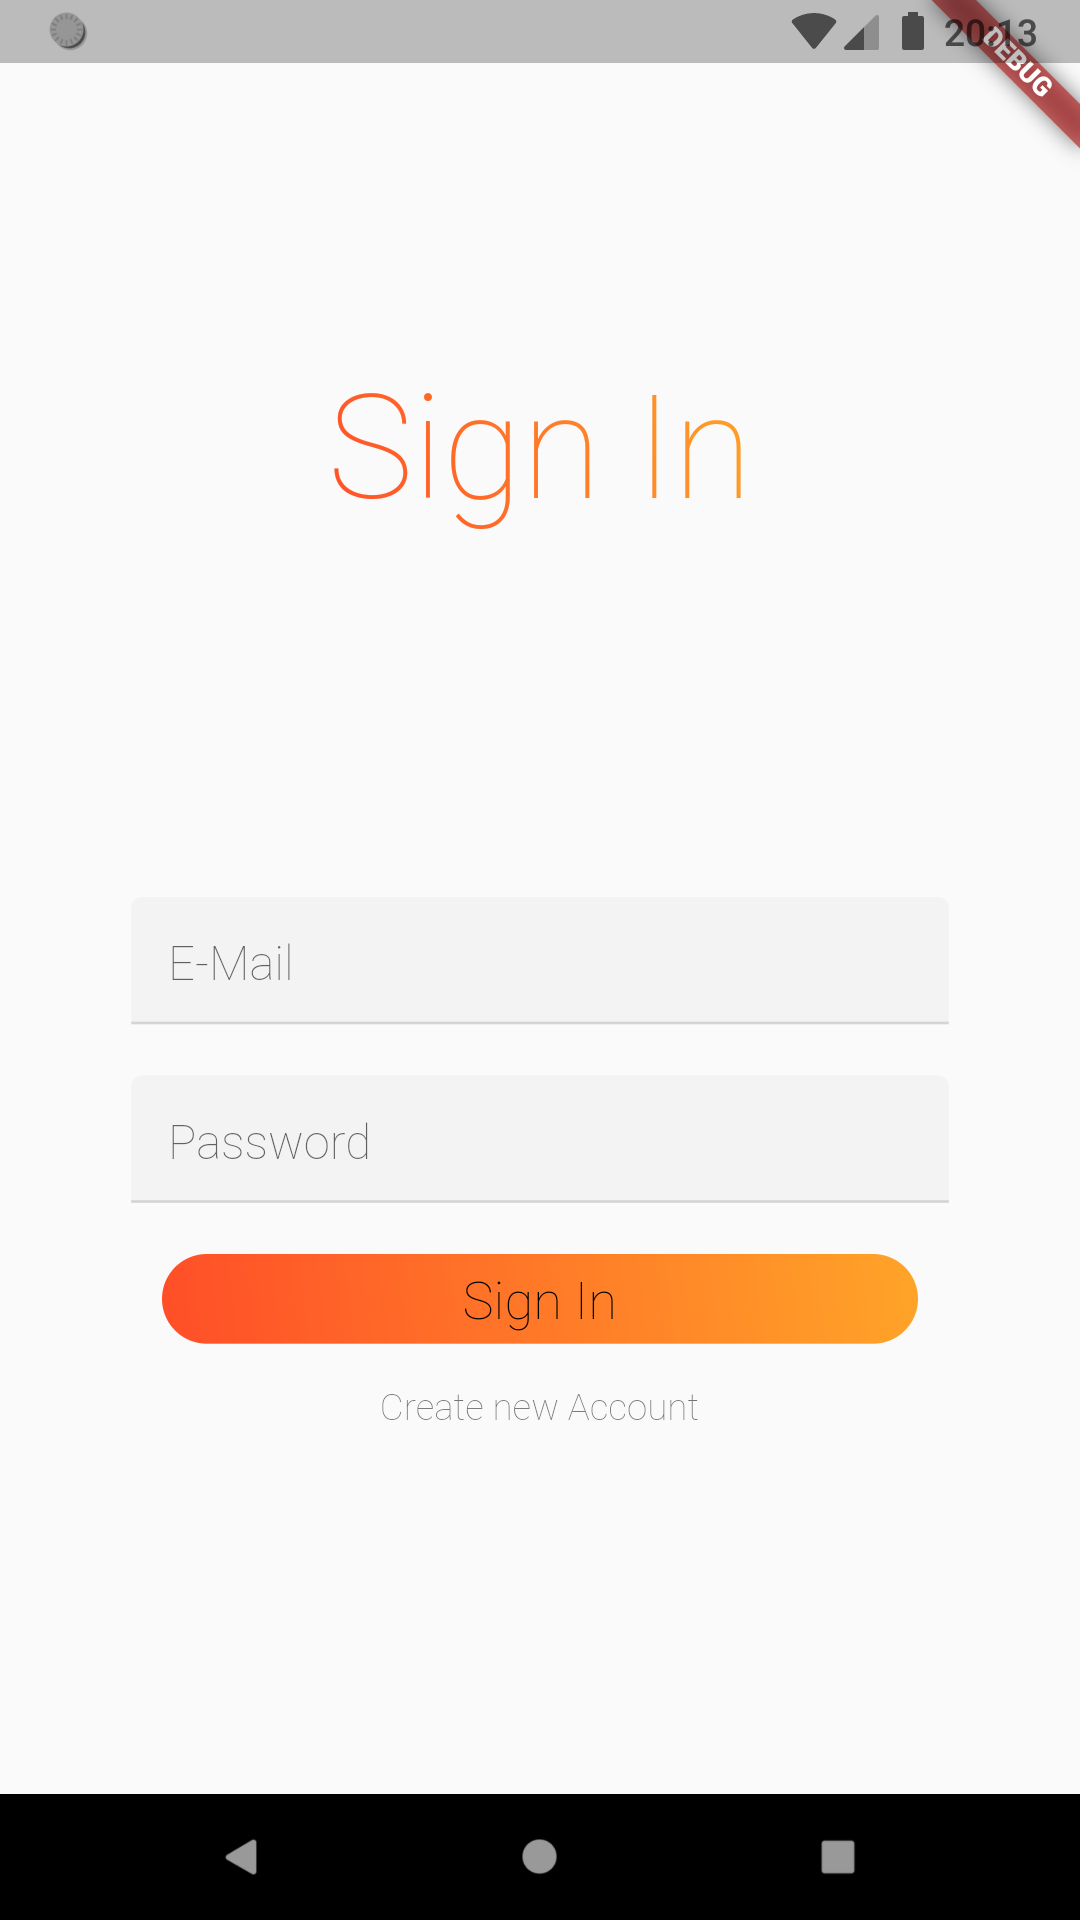
\includegraphics[scale=0.13]{Benutzeroberfläche/images/screenshot_login_1.png}
	\caption{}
	\label{fig:login_a}
	\end{subfigure}
	\begin{subfigure}{0.33\textwidth}
	\centering
	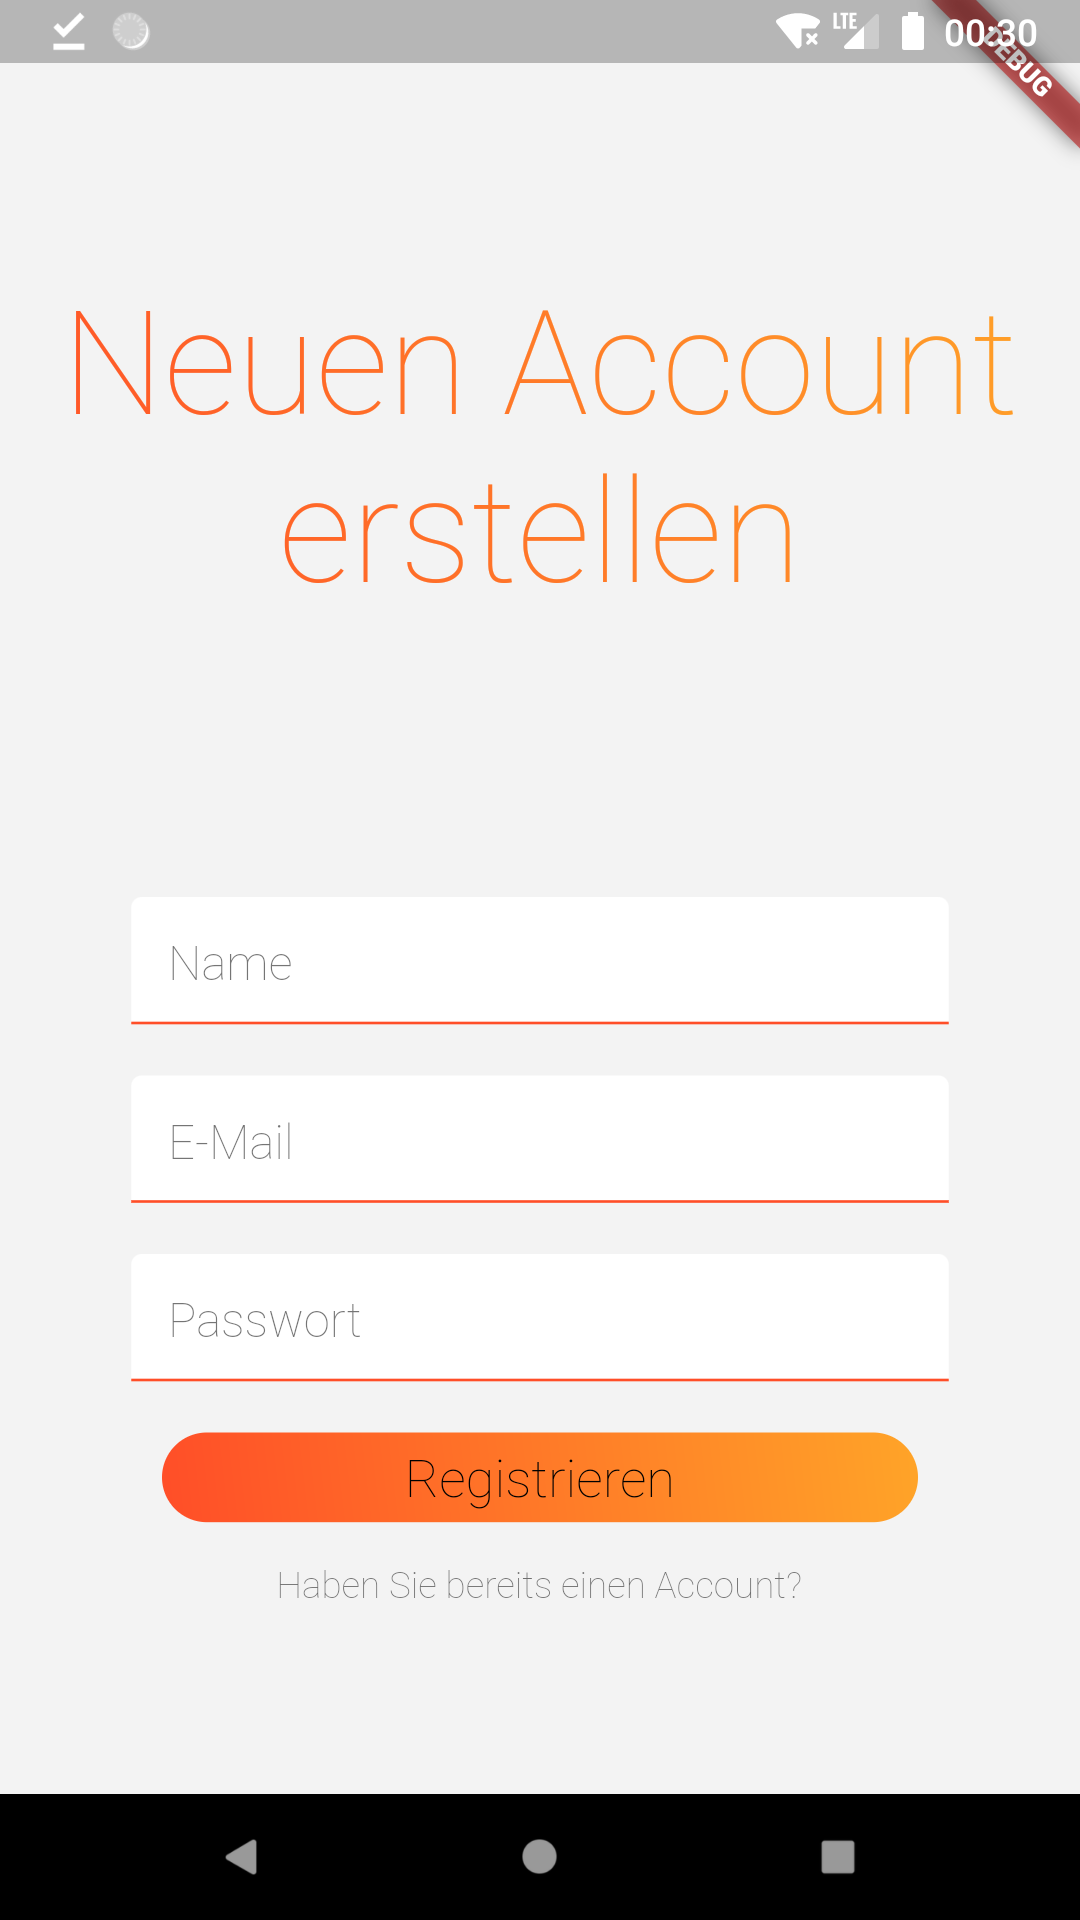
\includegraphics[scale=0.13]{Benutzeroberfläche/images/screenshot_login_2.png}
	\caption{}
	\label{fig:login_b}
	\end{subfigure}
	\begin{subfigure}{0.33\textwidth}
	\centering
	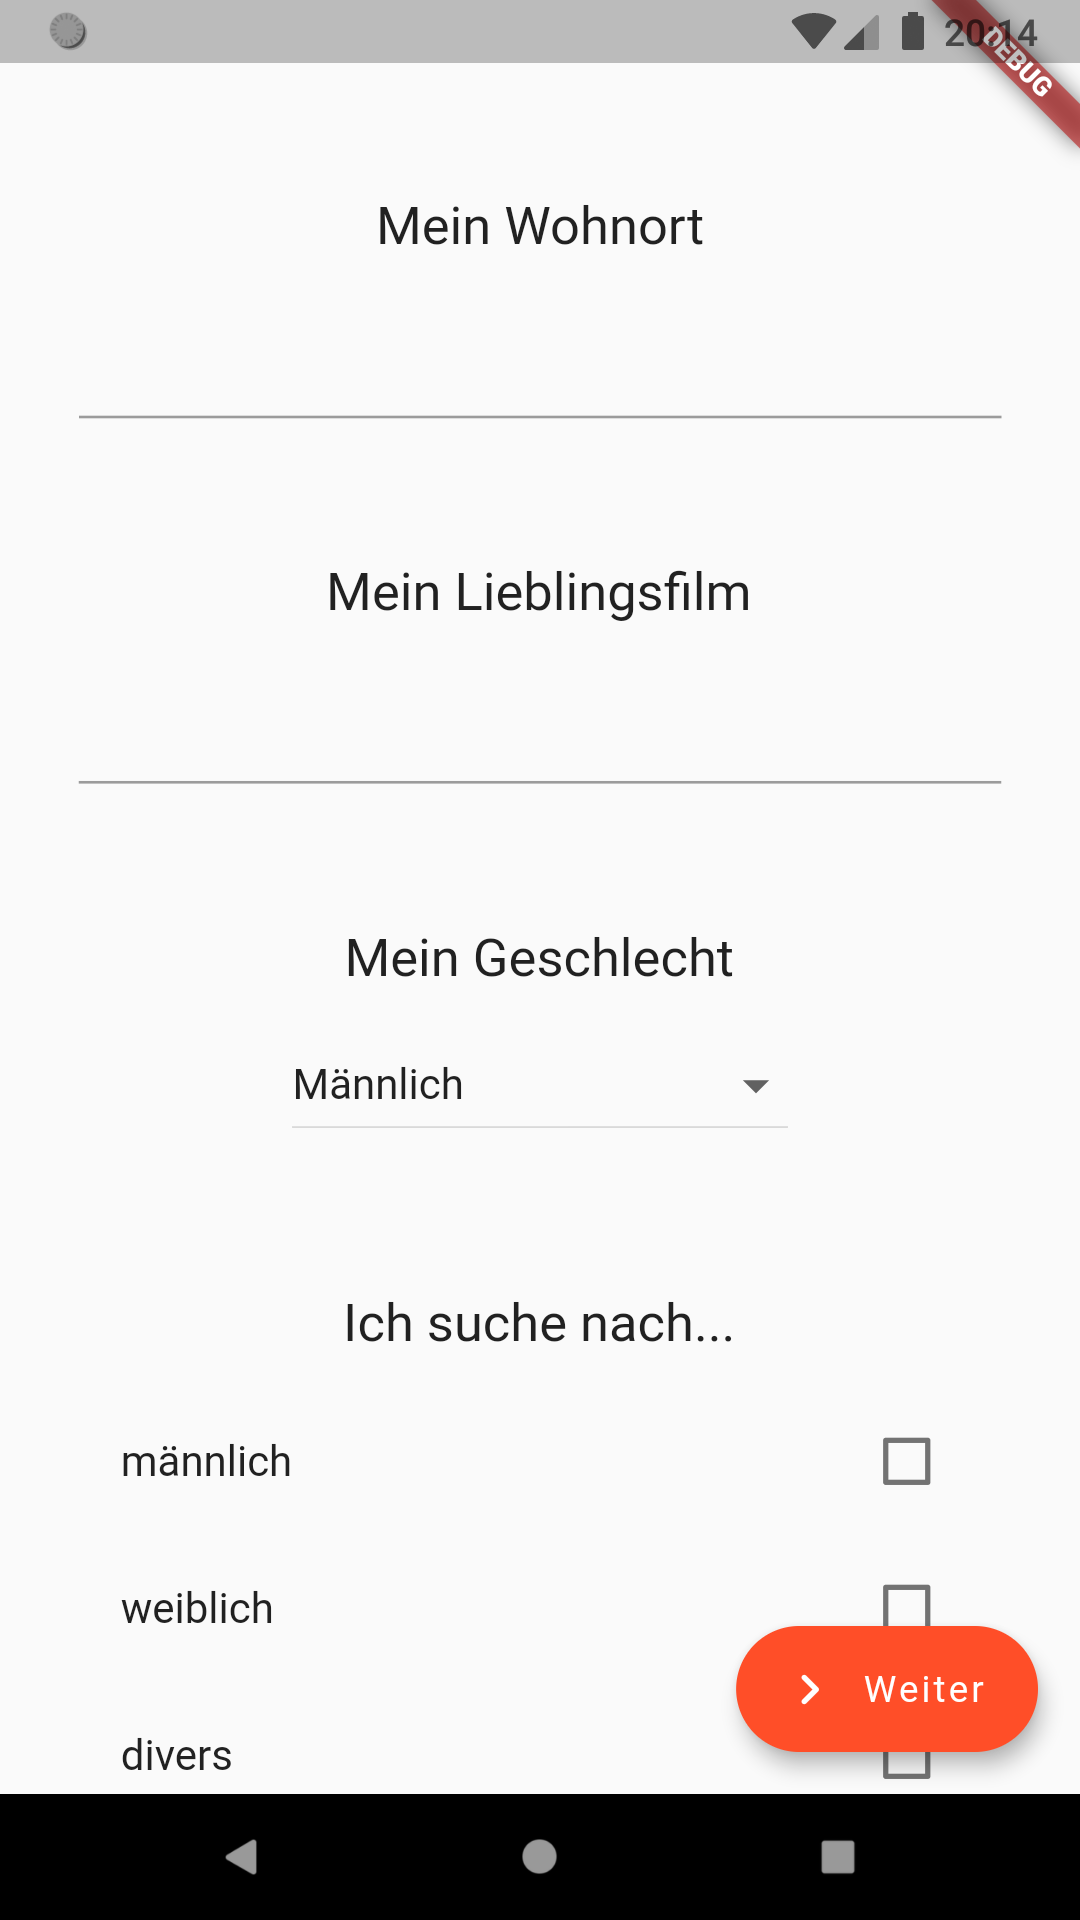
\includegraphics[scale=0.13]{Benutzeroberfläche/images/screenshot_login_3.png}
	\caption{}
	\label{fig:login_c}
	\end{subfigure}\\ \vspace{1cm}	
	
	\begin{subfigure}{0.33\textwidth}
	\centering
	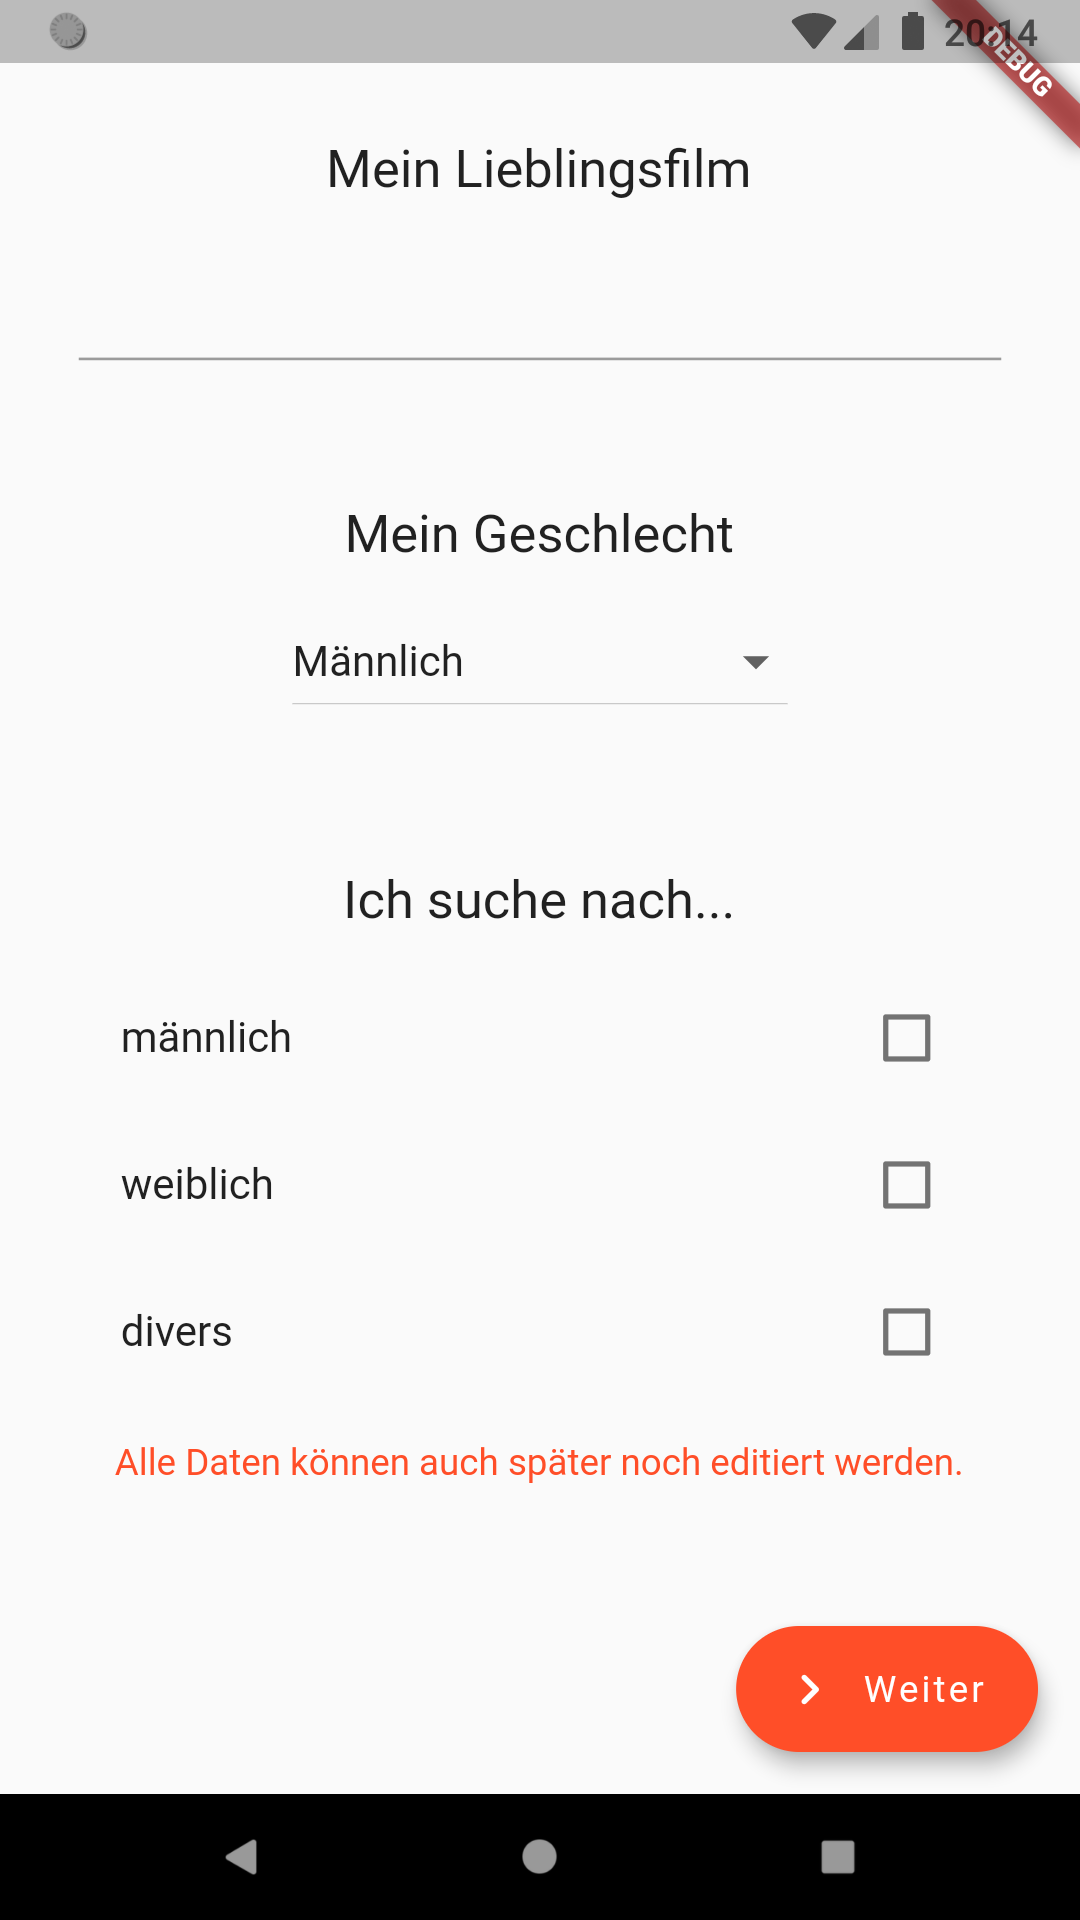
\includegraphics[scale=0.13]{Benutzeroberfläche/images/screenshot_login_4.png}
	\caption{}
	\label{fig:login_d}
	\end{subfigure}
	\begin{subfigure}{0.33\textwidth}
	\centering
	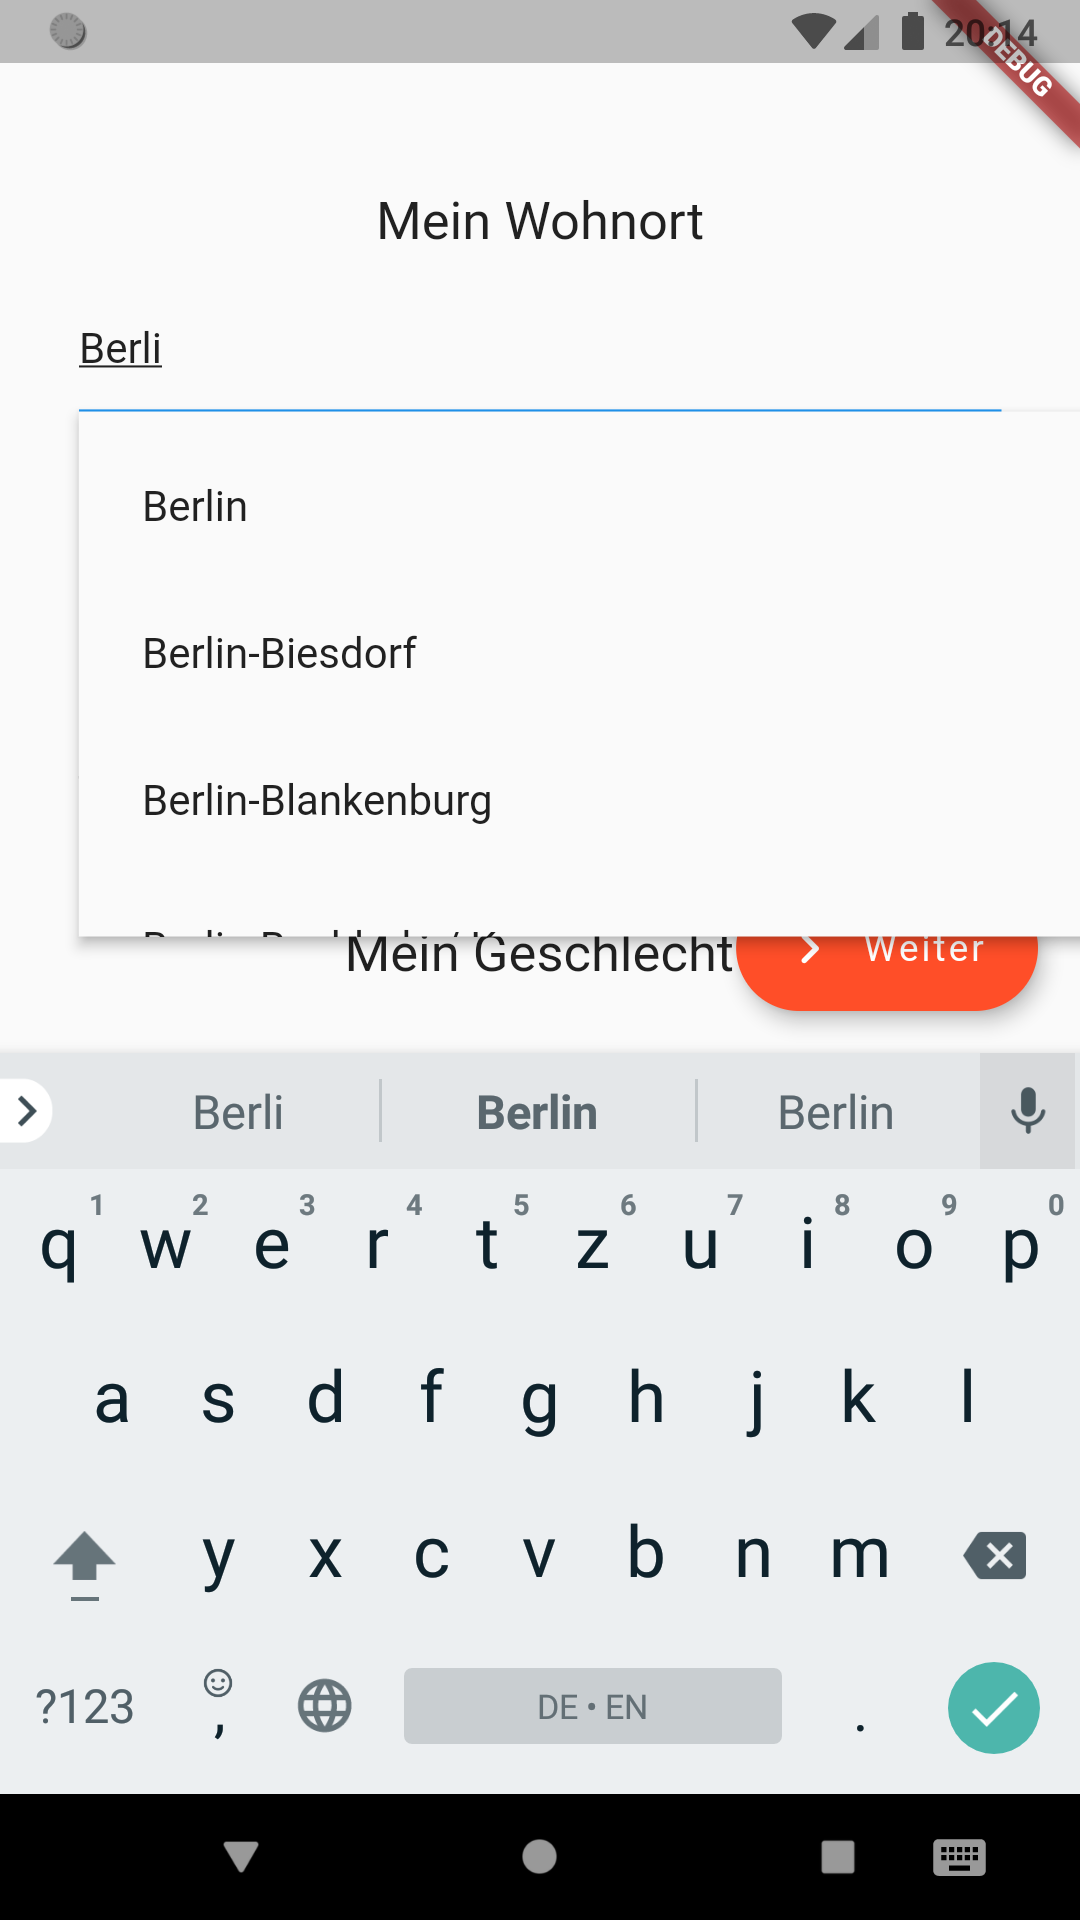
\includegraphics[scale=0.13]{Benutzeroberfläche/images/screenshot_login_5.png}
	\caption{}
	\label{fig:login_e}
	\end{subfigure}
	\begin{subfigure}{0.33\textwidth}
	\centering
	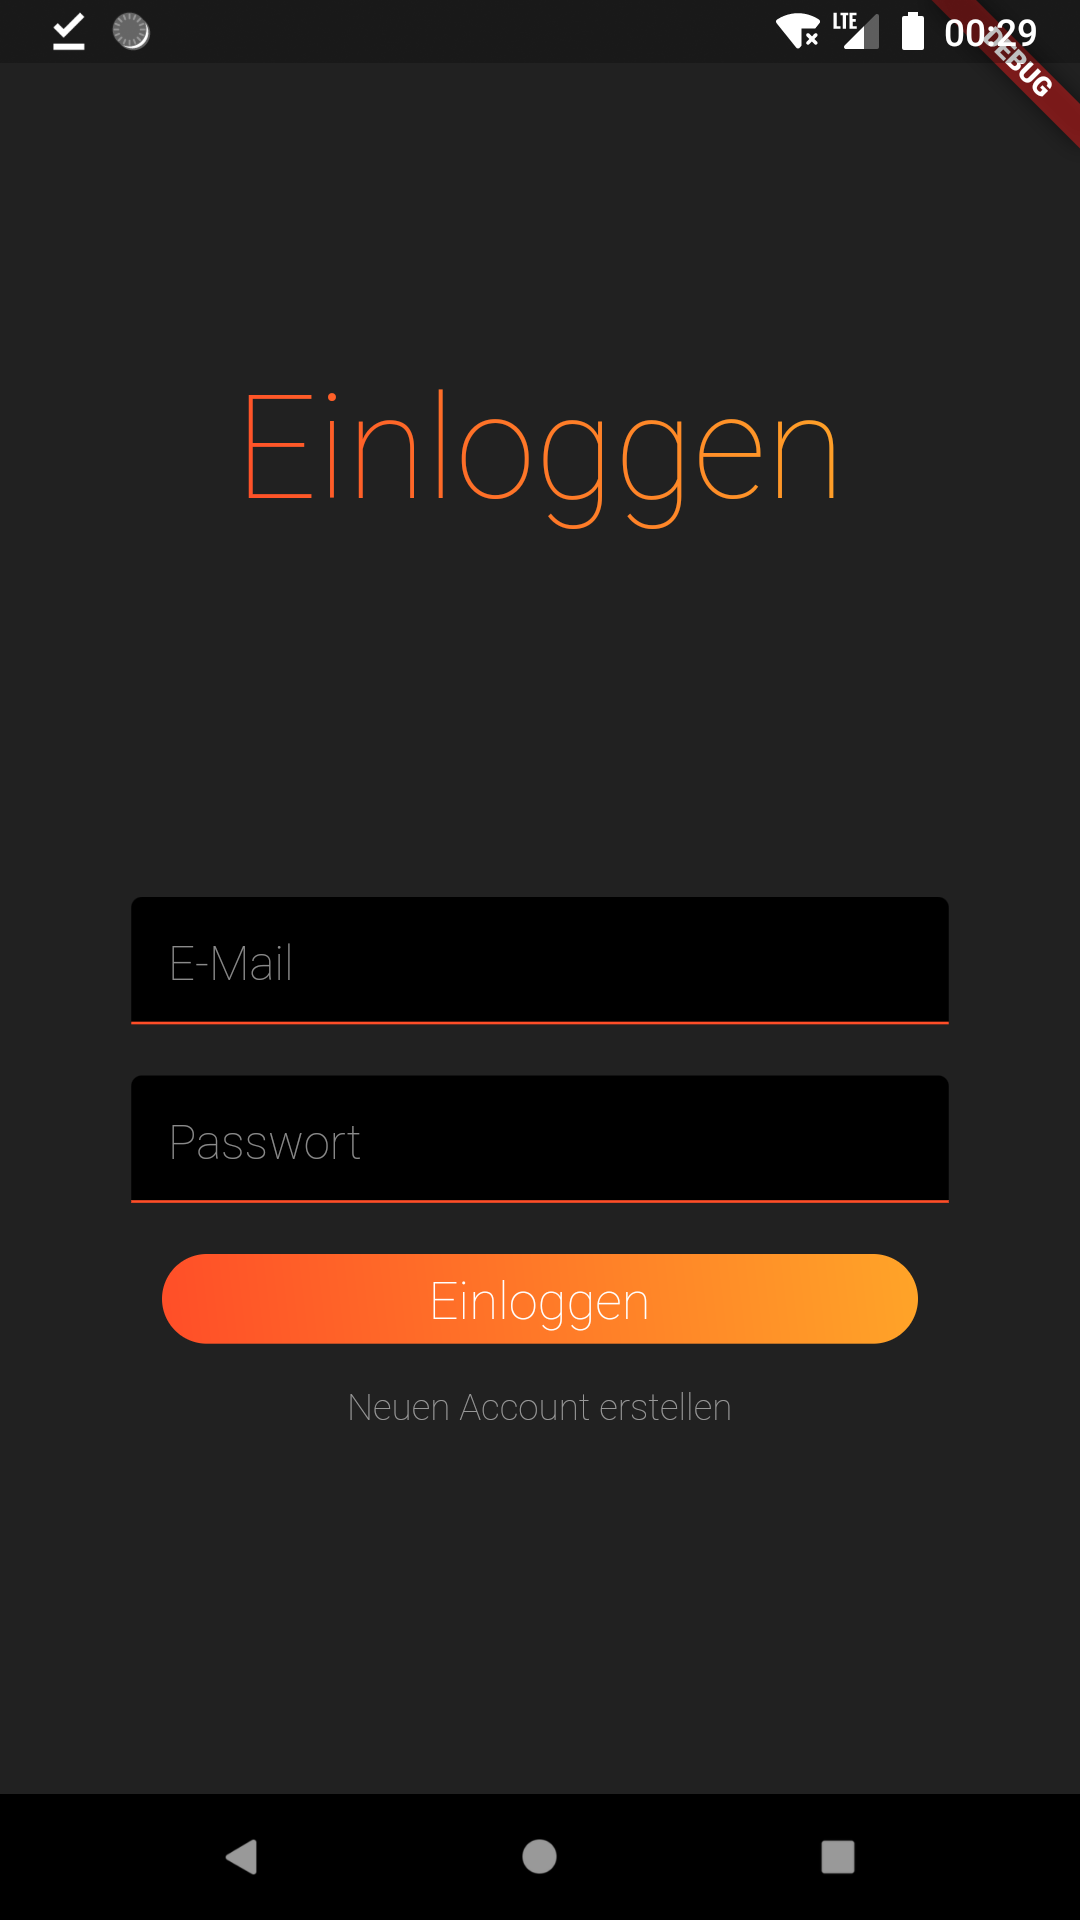
\includegraphics[scale=0.13]{Benutzeroberfläche/images/screenshot_darkmode_3.png}
	\caption{}
	\label{fig:login_f}
	\end{subfigure}
\caption[Screenshots der Anmeldeseiten]{Die Anmeldeseiten von StreamSwipe und alle damit zusammenhängenden Seiten. Man sieht (a) das Einloggen bei bestehendem Account, (b) das Erstellen eines Accounts, (c) und (d) das Formular für die benötigten Profildaten, (e) ein Texteingabefeld mit Autovervollständigung als Dropdownmenü und (f) das Farbschema der Anmeldeseiten im Darkmode am Beispiel der Login-Seite.}
\label{fig:login_alle}
\end{figure}
